
\begin{figure}[H]
\centering
\caption{Protótipo Interface Web - Tela de Login}
\label{fig:interface-web-tela-login}
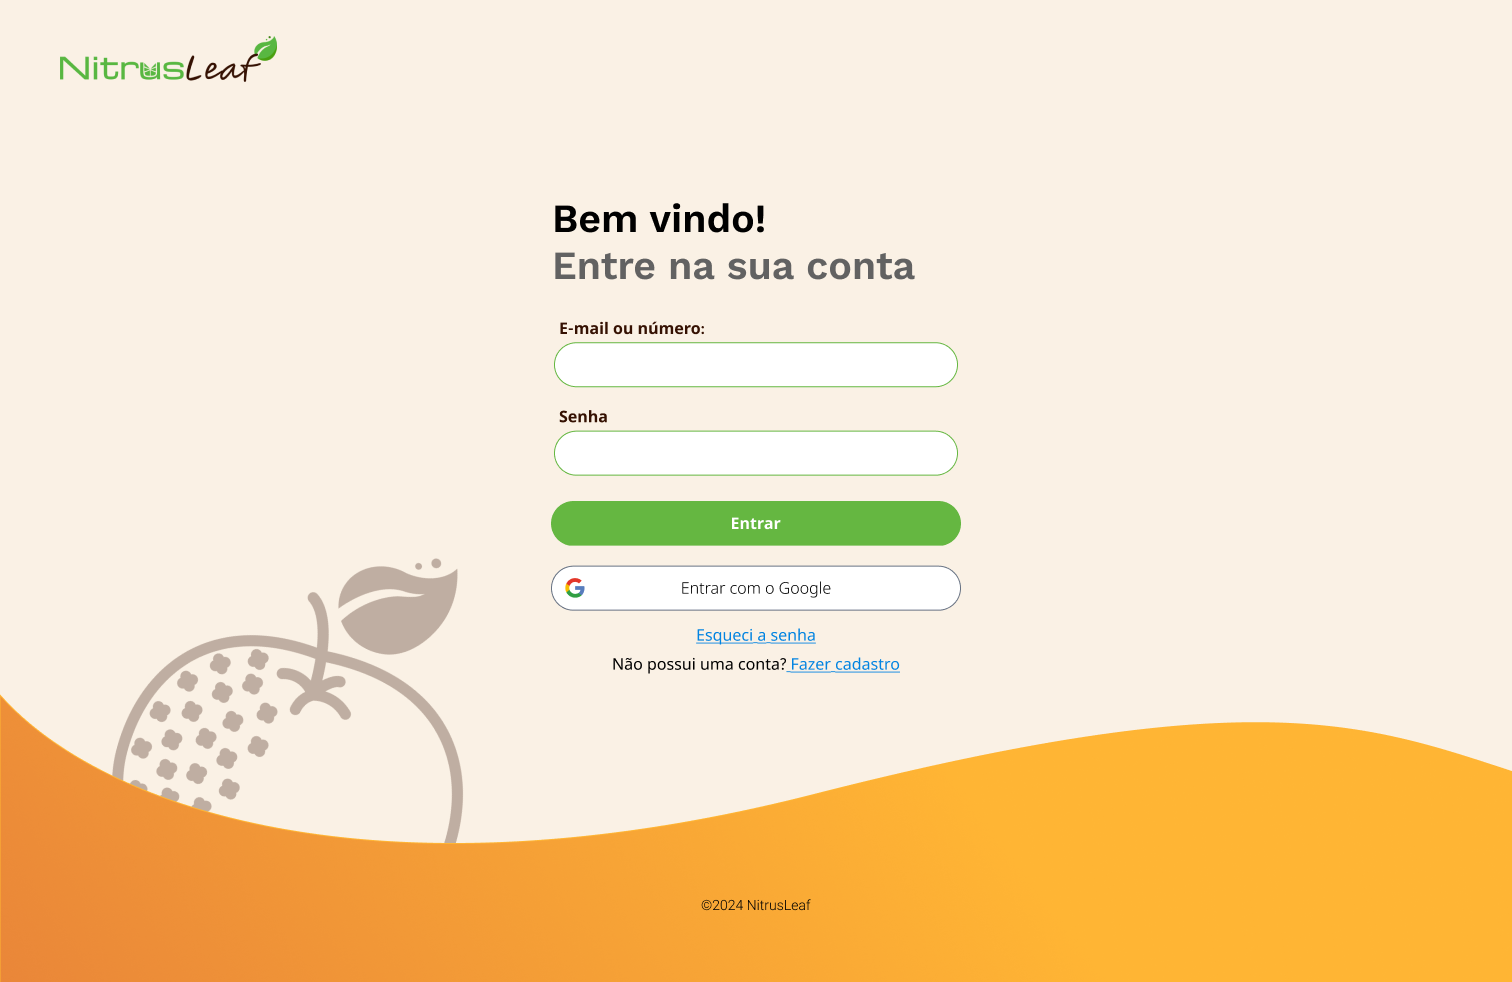
\includegraphics[width=0.8\textwidth]{Images/TelaLogin.png}
\SourceOrNote{Equipe 21 - Vitalliz (2025)}
\end{figure}

A tela de login é o ponto de entrada do sistema. Ela permite o acesso de usuários
previamente cadastrados, garantindo segurança e controle de acesso às
funcionalidades do sistema.
\medskip


\begin{figure}[H]
\centering
\caption{Protótipo Interface Web - Tela de Histórico}
\label{fig:interface-web-telahistorico-1}
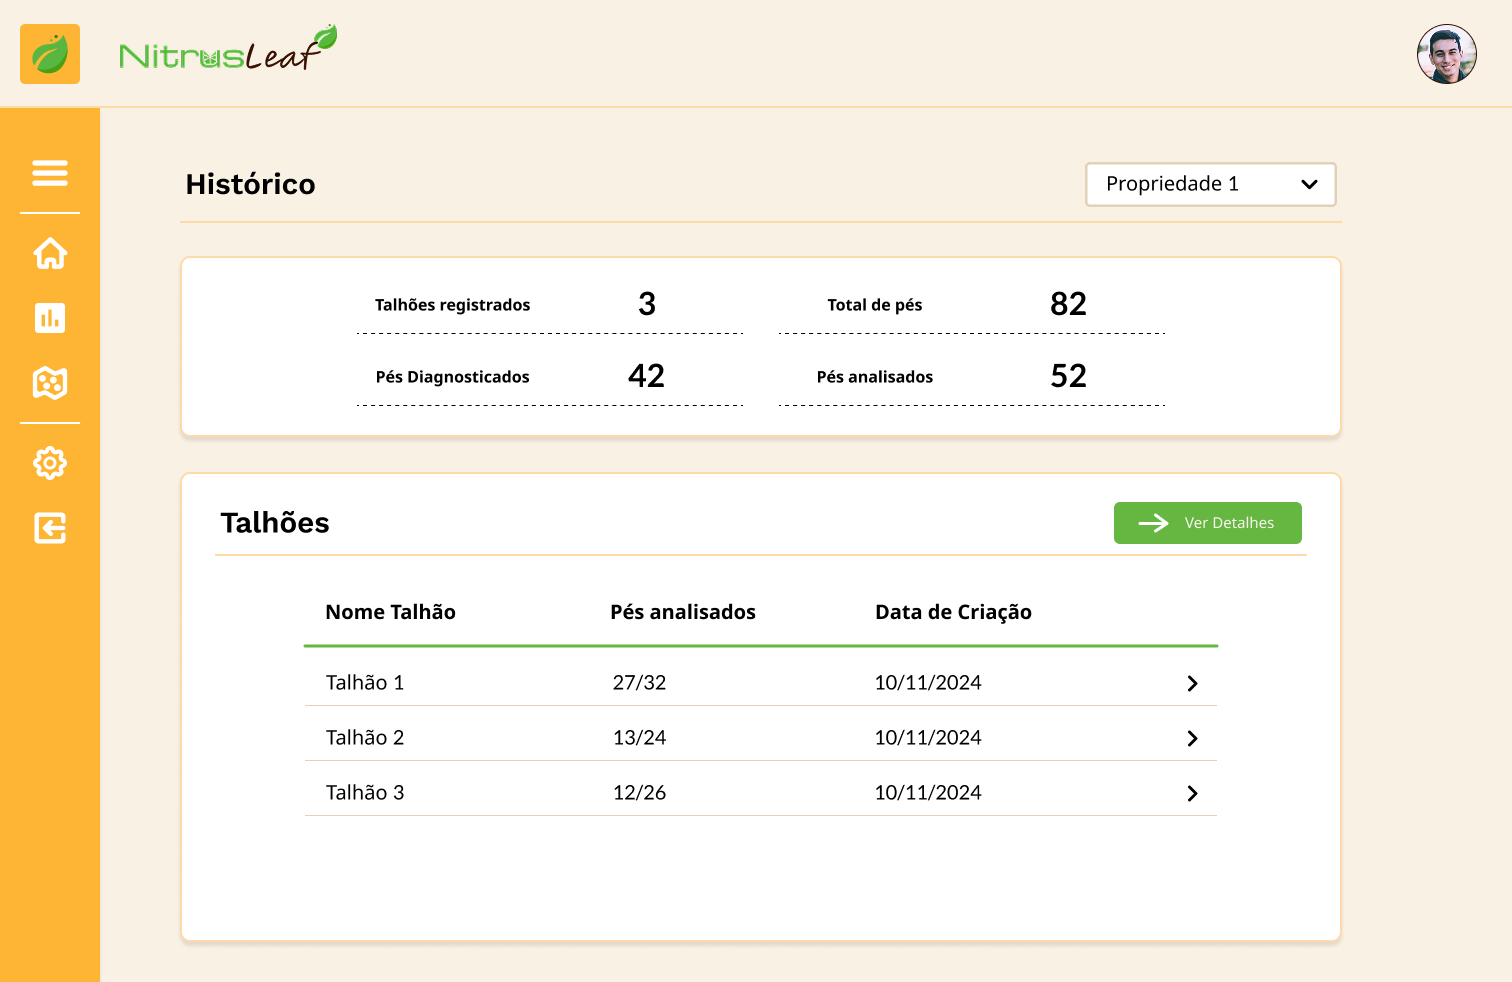
\includegraphics[width=0.8\textwidth]{Images/TelaHistorico-1.png}
\SourceOrNote{Equipe 21 - Vitalliz (2025)}
\end{figure}

A tela de histórico apresenta registros anteriores de análises feitas em cada
talhão, permitindo o acompanhamento da evolução das deficiências identificadas,
datas de envio das imagens e resultados processados.
\medskip


\begin{figure}[H]
\centering
\caption{Protótipo nterface Web - Tela de Resultados}
\label{fig:interface-web-tela-resultados}
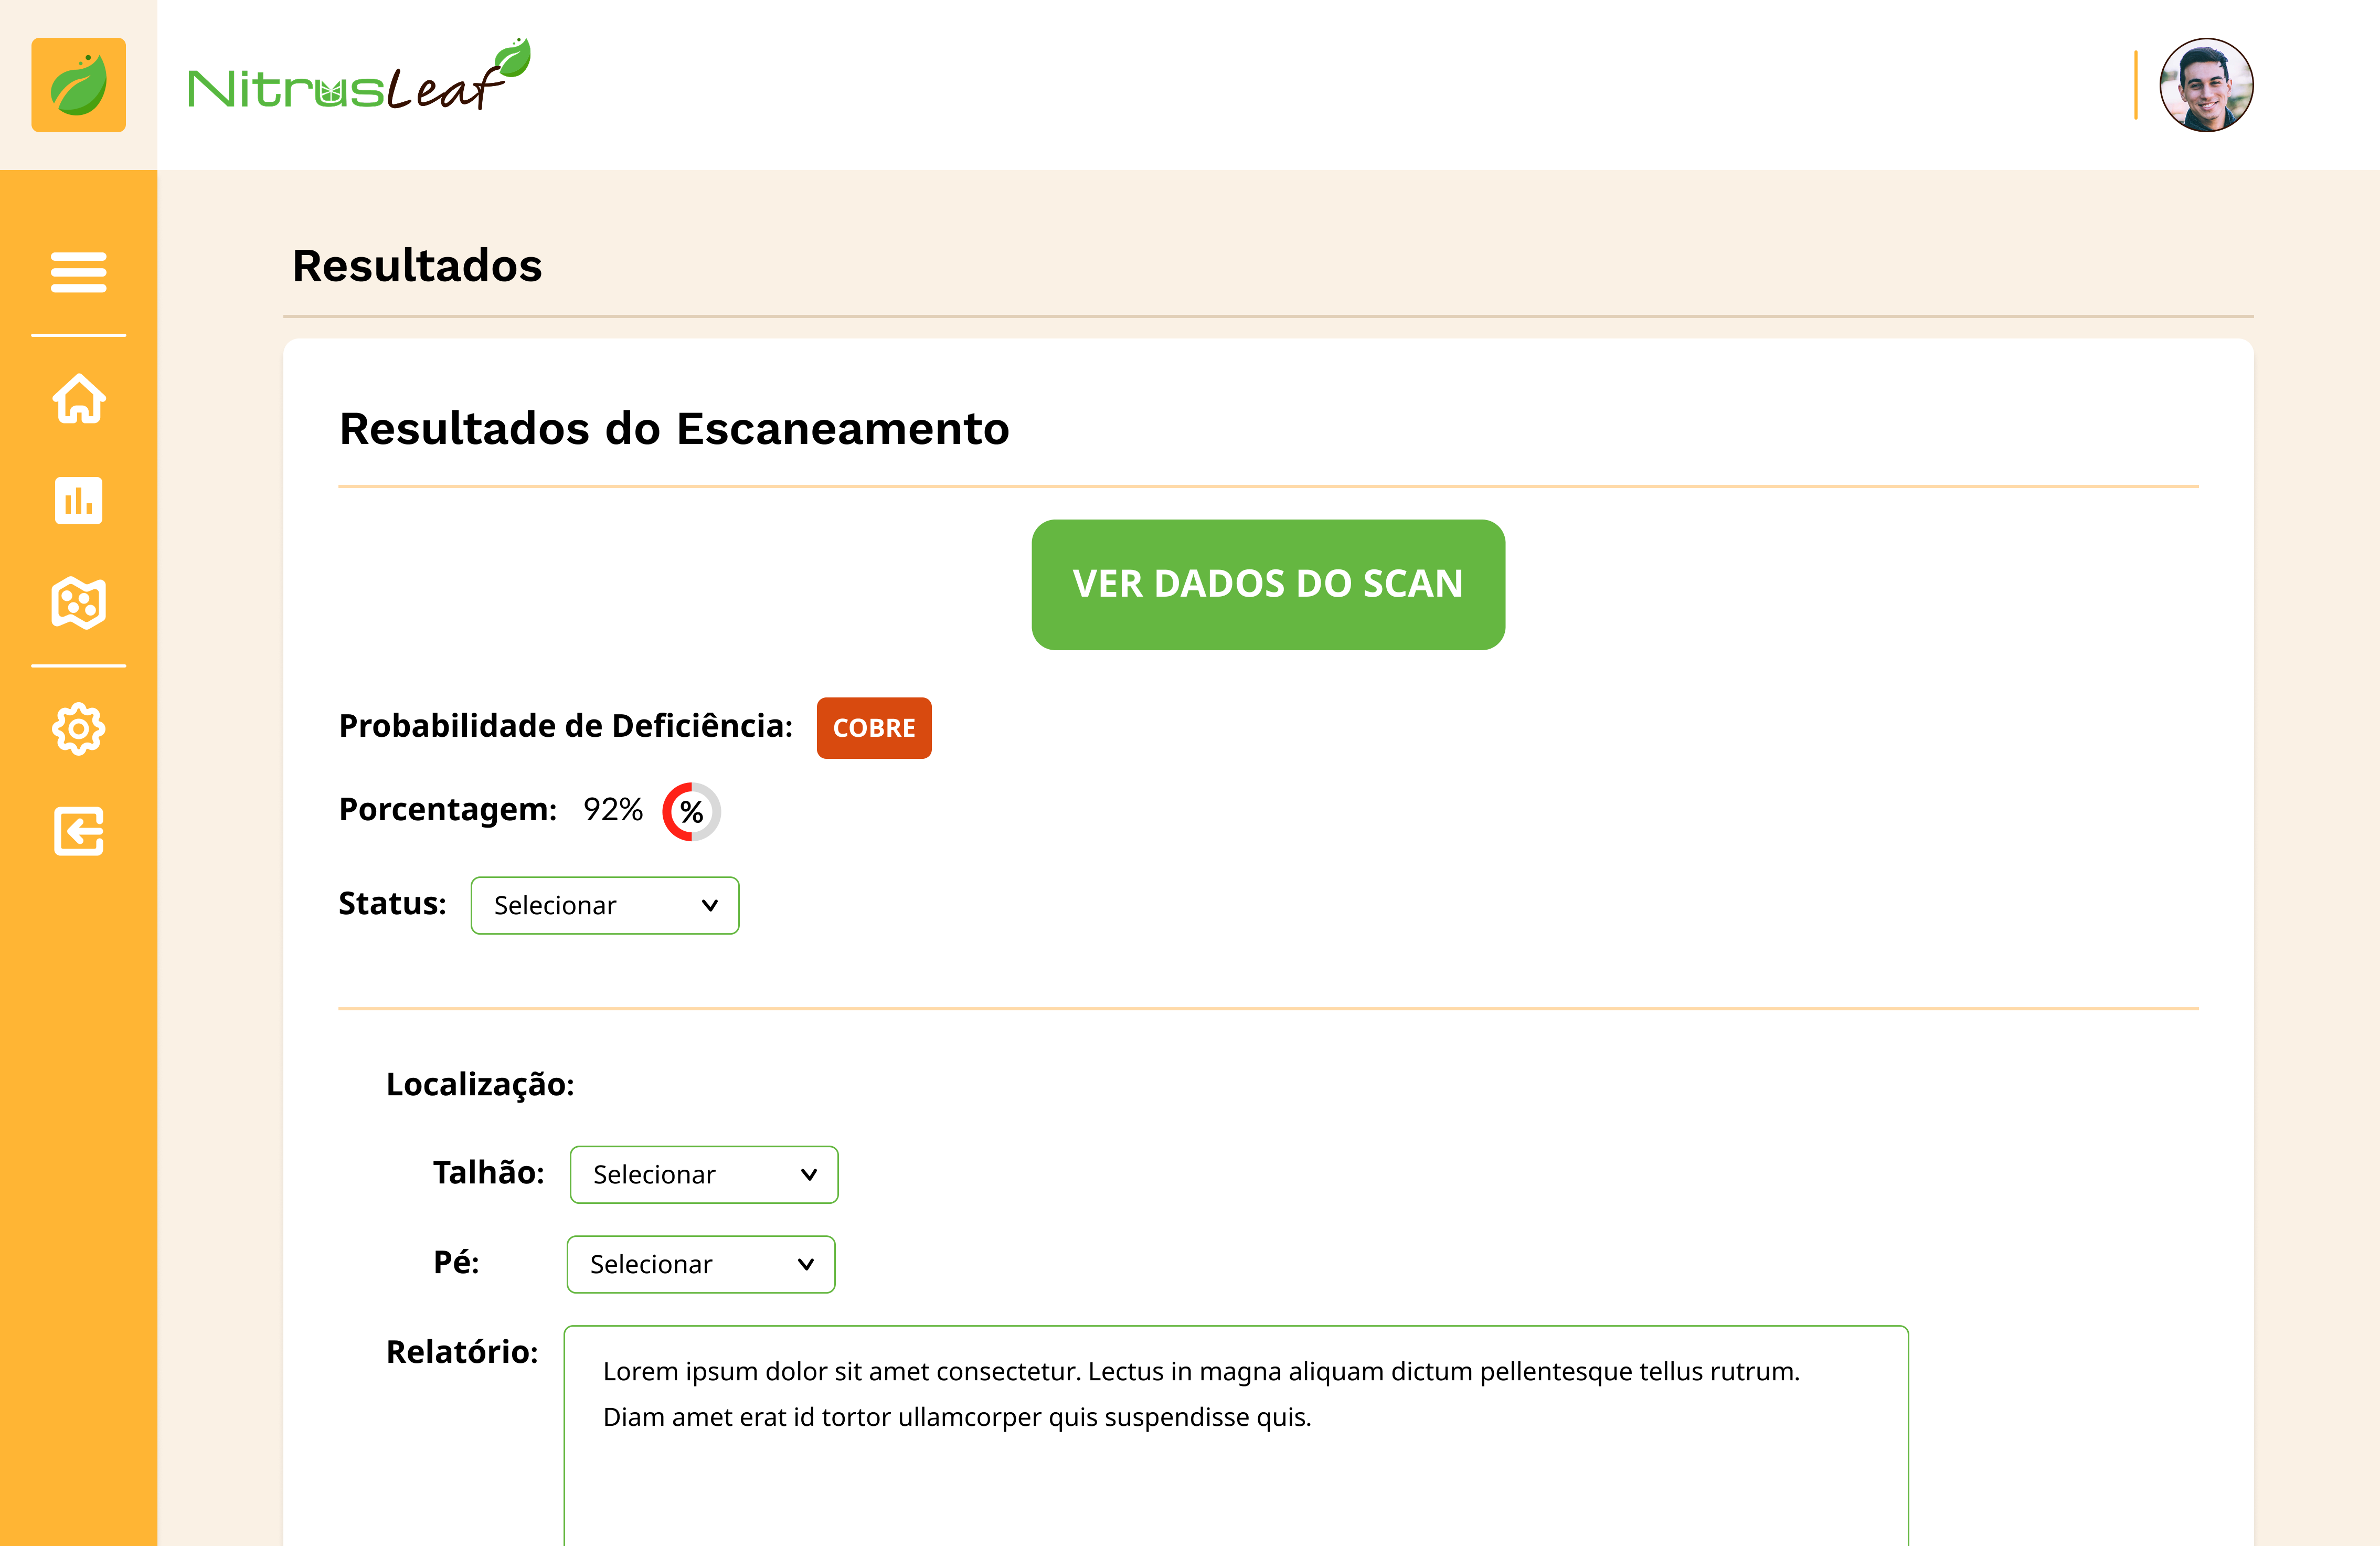
\includegraphics[width=0.8\textwidth]{Images/TelaResultado.png}
\SourceOrNote{Equipe 21 - Vitalliz (2025)}
\end{figure}

A tela de Resultados exibe os resultados detalhados das análises realizadas nas
imagens enviadas, incluindo definição de status e criação de relatórios.
\medskip


\begin{figure}[H]
\centering
\caption{Protótipo Interface Web - Tela de Mapa}
\label{fig:interface-web-tela-mapa}
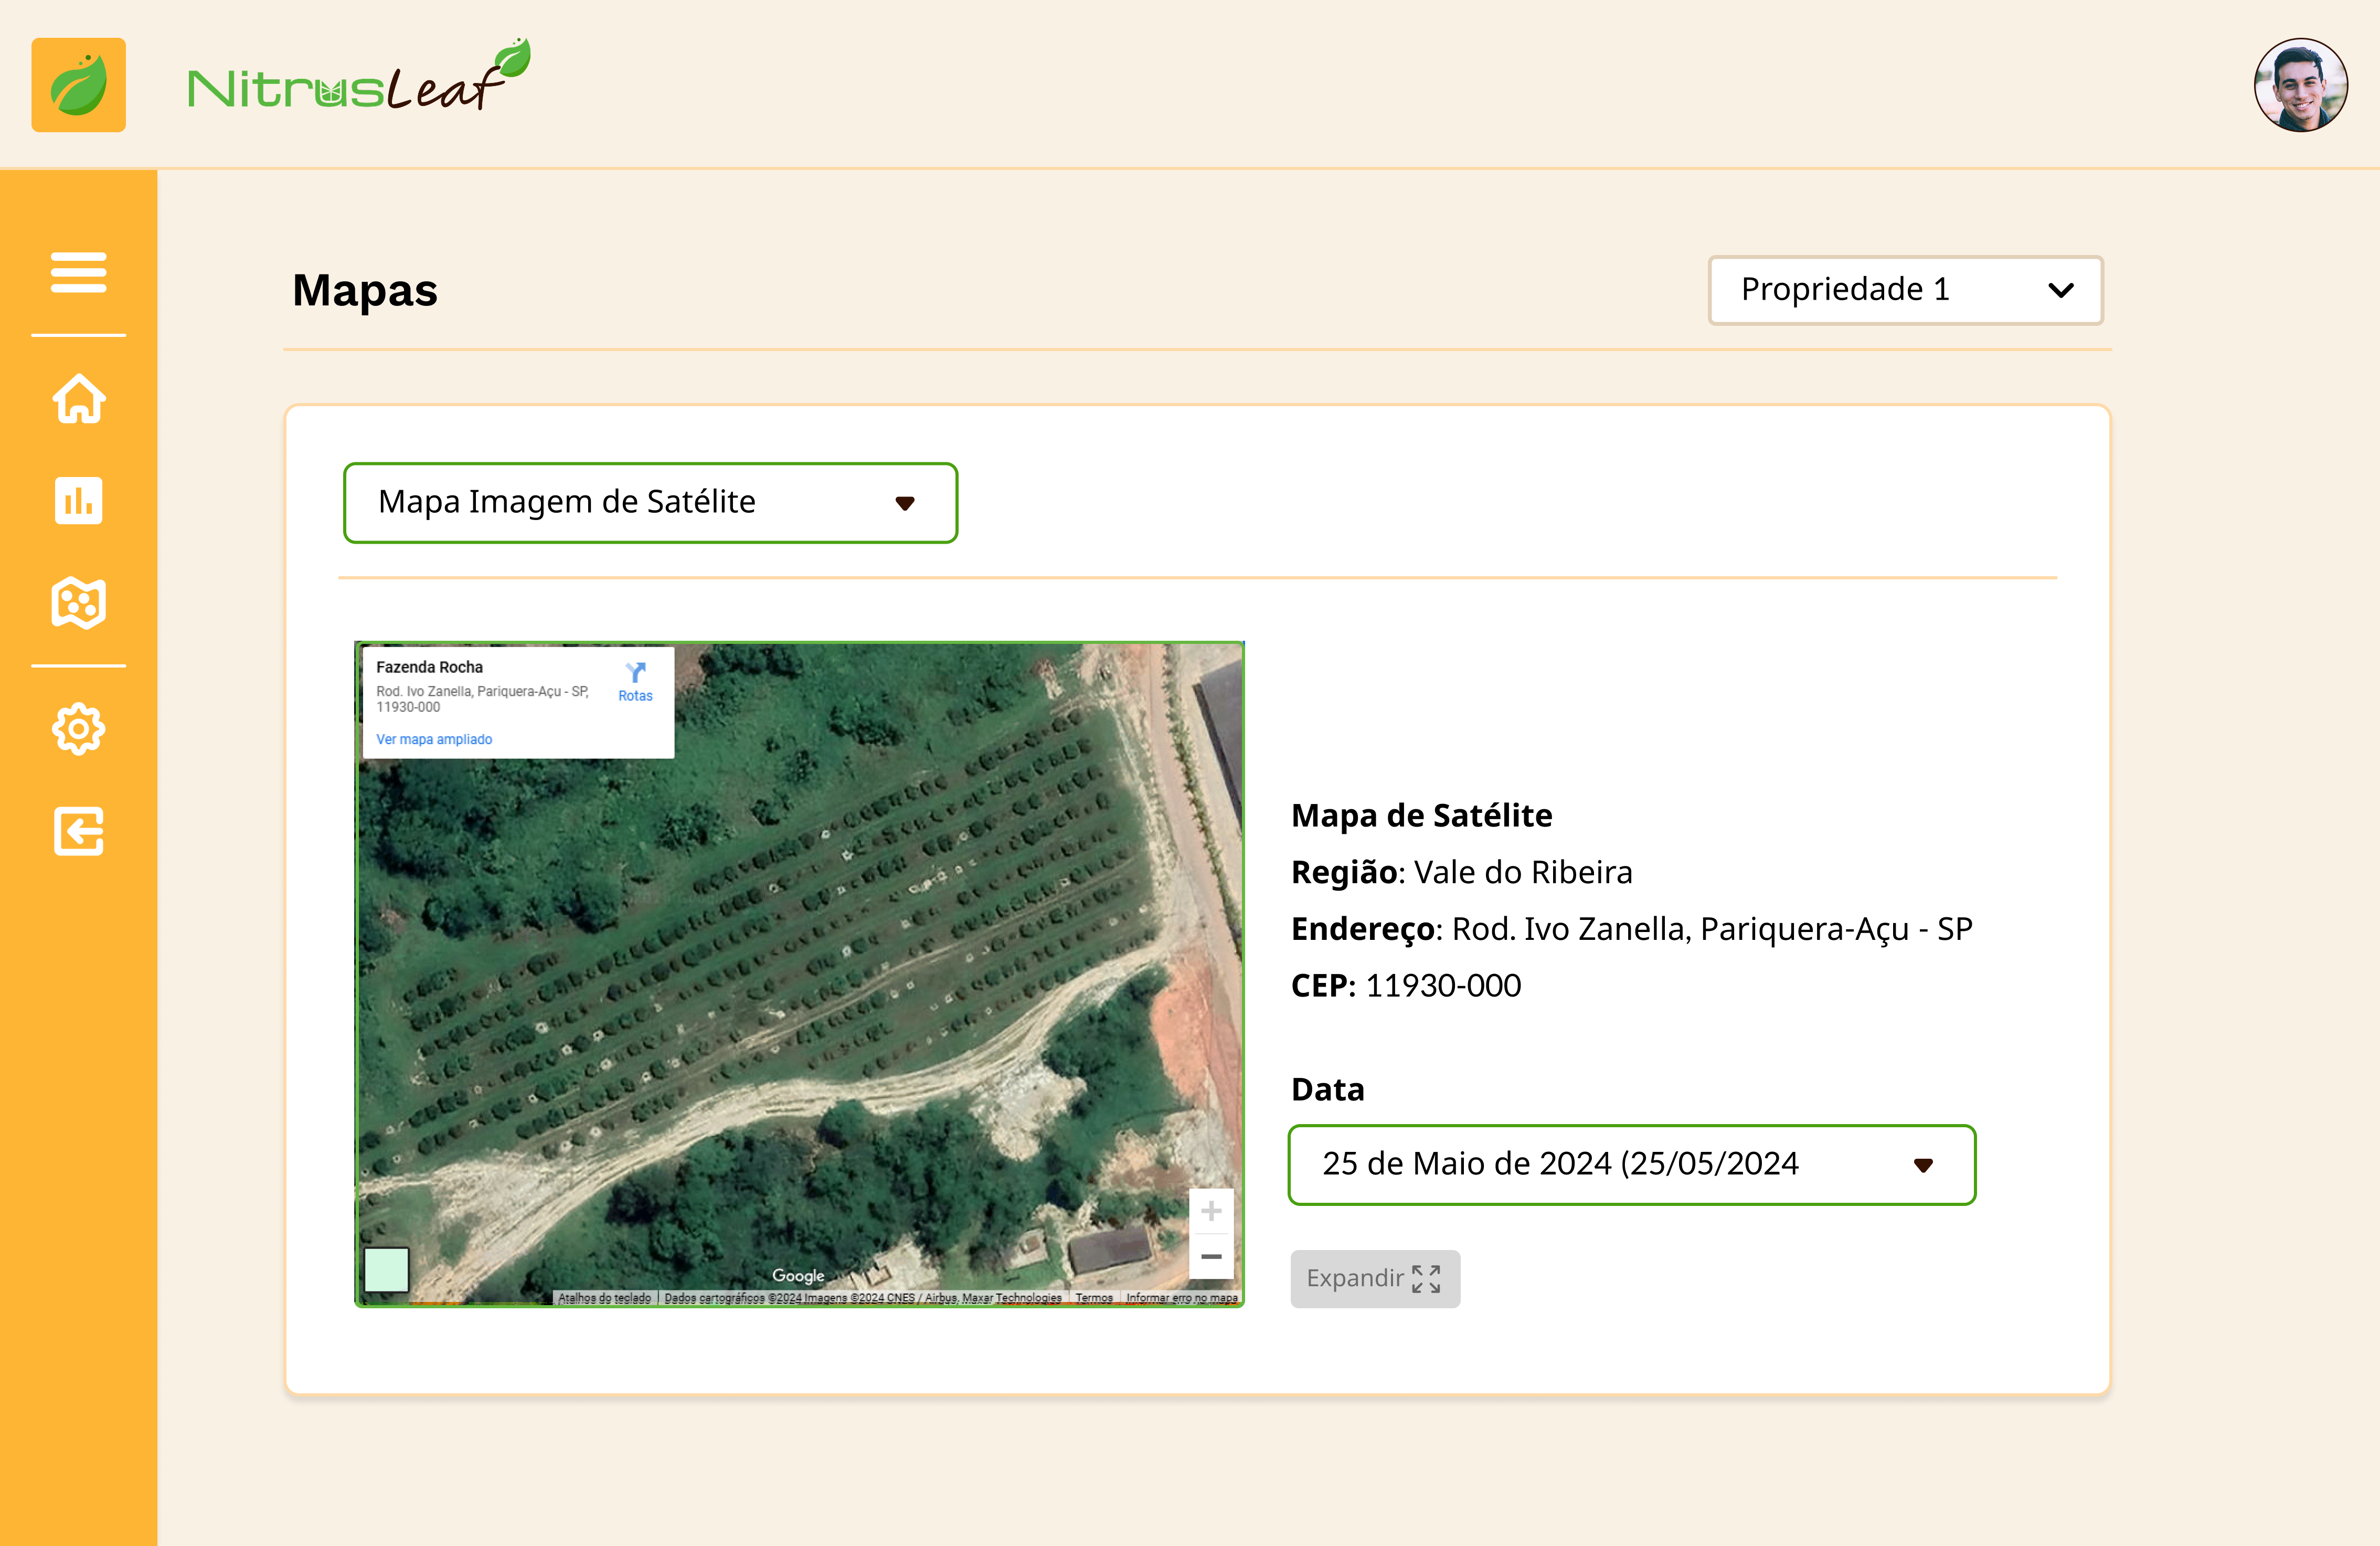
\includegraphics[width=0.8\textwidth]{Images/TelaMapa.png}
\SourceOrNote{Equipe 21 - Vitalliz (2025)}
\end{figure}

Nesta tela, o usuário pode visualizar os talhões de sua propriedade em um
mapa interativo.
\medskip